\documentclass[11pt]{report}
\usepackage{geometry}                % See geometry.pdf to learn the layout options. There are lots.
\geometry{a4paper}                   % ... or a4paper or a5paper or ... 
\usepackage{listings}
%\usepackage[parfill]{parskip}    % Activate to begin paragraphs with an empty line rather than an indent
\usepackage{graphicx}
\usepackage{amssymb}
\usepackage{epstopdf}
\usepackage[usenames, dvipsnames]{color}
\usepackage{hyperref}

\DeclareGraphicsRule{.tif}{png}{.png}{`convert #1 `dirname #1`/`basename #1 .tif`.png}

\newcommand{\leongage}{NoBeard}

\newenvironment{grammar}
	{\begin{tabular}[b]{lcl}}
	{\end{tabular}}
\newcommand{\rewritten}{$\to$}
\newcommand{\alternative}{$\mid \;$}
\newcommand{\emptystring}{$\varepsilon$}

\newenvironment{atg}[1][6cm]
	{\begin{tabular}[b]{lclp{#1}}}
	{\end{tabular}}
\newcommand{\atgsy}[2]{$\textrm{#1}_\textrm{#2}$}
\newcommand{\outattr}{$\uparrow$}
\newcommand{\inattr}{$\downarrow$}

\newcommand{\semantics}[1]{\textcolor{Gray}{#1}}

\newenvironment {sem}
	{\underline{sem}}
	{\underline{endsem}}
	
\newcommand{\where}{\underline{where} }

\author{P. Bauer}
\date{V.\_01.00.00}                                           % Activate to display a given date or no date

\lstdefinelanguage{NoBeard}{
	morekeywords = {unit, function, do, done, int, char},
	sensitive=false,
	morecomment=[l]{\#}
}

\begin{document}
\begin{titlepage}
\begin{center}

\includegraphics[scale=0.3]{no_beard_1.jpg} \\[2em]
%\includegraphics[scale=0.3]{no_beard_2.jpg} \\[2em]
{\Huge A Formal Description of \leongage} \\[1em]
{\large v 01.01.00} \\[2em]
{\Large P. Bauer} \\[1em]
HTBLA Leonding \\
Limesstr. 14 - 18 \\
4060 Leonding \\
Austria
\end{center}
\end{titlepage}

%\maketitle
\tableofcontents
\chapter{Introduction}
According to a web article (see \cite{khason_computer_2008}) the popularity of programming languages is strongly related to the fact whether its inventor(s) is/are are bearded m[ae]n or not. Well, the main aim of the programming language \leongage{} is not to be popular,
moreover it should give the reader a clear insight how the main principles of compiler construction are.

This report aims to give a formal description of the programming language \leongage. Please note that only the parts
necessary for your work can be trusted. In the next versions, more and more information relevant for your assignments
will be available.

In case of typos, misleading wording or other problems, please feel free to contact me. Thanks for your help. Some more text to read~\cite{terry_compiling_2004}. 

\chapter{The Programming Language}
\section{Lexical Structure}

\leongage{} programs are written in text files of free format, i.e., there is no restriction concerning columns or lines where
the source text has to be. In this section the scanner relevant terms for \leongage{} are denoted in the form of regular expressions
with the extension that we allow "definitions" of non-terminals. This means in particular that if we define a term (e.g.
{\em letter} as it can be seen in the next section) this term can be used in subsequent definitions and is rewritten as
given in its original definition.

\subsection{Character Sets}
\begin{description}
	\item[letter] \texttt{'[A-Za-z]'}
	\item[digit]\texttt{'[0-9]'}
\end{description}

\subsection{Keywords}
There is only one keyword, namely \texttt{PUT}.

\subsection{Token Classes}
\begin{description}
	\item[ident] \texttt{['letter(letter \alternative digit)*']}
	\item[number] \texttt{['digit digit*]}
\end{description}

\subsection{Single Tokens}
The characters "{\tt+}", "{\tt-}", "{\tt*}", "{\tt/}", "{\tt:=}", "{\tt;}", "{\tt(}", and "{\tt)}" are mapped to single tokens.

\subsection{Semantics}
\begin{itemize}
	\item \leongage{} is a case sensitive language. For example, the names "myVar", "myvar", and "MYVAR" denote three different identifiers.
	\item Constants may only be between 0 and 65535 ($2^{16} - 1$).
	\item No symbol may span over more than one line.
\end{itemize}

\section{Sample Program}
\begin{lstlisting}
unit ComplexExpr;
# ---------------------------- ComplexExpr.nb -----------
# --- A syntactically correct NoBeard program
# -------------------------------------------------------
do
    int l = 10;
    int b =5;
    int h= 170;
        int unused = l;
    int x=1001 + l * b - h / (b * h);

    put ("Evaluating 1001 + l * b - h / (b * h)");
    putln;
    put ("Result is ");
    put (x);          # result should be 1051
done ComplexExpr;
\end{lstlisting}

\section{Syntax}
The following context free grammar gives the syntax of \leongage{}. The well-known EBNF notation~\cite{wirth_what_1977} is used.

	\begin{grammar}
	NoBeard & = & ``unit" ident ``;" Block ident ``;".\\
	
	Block & = &  ``do" StatSeq ``done".\\
	
	StatSeq & = & Stat \{Stat\}. \\
	
	Stat & = & VarDecl ``;" \\
%	&& \alternative FuncDecl ";" \\
	&& \alternative Assignment ``;"\\
%	&& \alternative FuncCall ";" \\
	&& \alternative PutStat ``;" \\
%	&& \alternative IfStat \\
	&& \alternative \emptystring. \\
	
	VarDecl & = & Type ident [``=" Expr]. \\
	
	Type & = & SimpleType [ArraySpec]. \\
	
	%TypeSpec & = & SimpleType %\alternative CompoundType. \\
	
	ArraySpec & = & ``[" number ``]". \\
	
	SimpleType & = & ``int" \alternative ``char" \alternative ``bool". \\
	
%	FuncDecl & = & "function" ReturnType ident ["(" FormalArguments ")"] Block ident. \\
	
%	ReturnType & = & TypeSpec  [ArgArraySpec]. \\
	
%	ArgArraySpec & = & "[" "]". \\
	
%	FormalArguments & = & Argument \{"," Argument\}. \\
	
%	Argument & = & TypeSpec [ArgArraySpec] ident. \\
	
	Assignment &=& Reference ``=" Expr . \\
	
%	FuncCall & = & ident ["(" Expr \{"," Expr\}]. \\

%	IfStat & = & ``if" Expr Block \\
%	&& [``else" Block]. \\
	
%	WhileStat & = & "while" "[" CondExpr "]" "do" StatSeq "done". \\
	
	PutStat & = & ``put" ``(" Expr [``," Expr] ``)" \\
	&& \alternative "putln". \\
	
	Expr & = & SimExpr [RelOp SimExpr]. \\
	
	SimExpr & = & [AddOp]Term \{AddOp Term\}. \\
	
	Term & = & Fact \{MulOp Fact\}. \\
	
	Fact & = & Reference \alternative number \alternative string \\
	&& \alternative %FuncCall \alternative
	``(" Expr ``)". \\
	
	Reference & = & ident [ ``[" Expr ``]"]. \\
	
	RelOp & = & "$<$" \alternative "$<$=" \alternative "==" \alternative "!=" \alternative "$>$=" \alternative "$>$". \\
	
	AddOp & = & ``+" \alternative ``-". \\
	
	Mulop & = & ``*" \alternative ``/" \alternative ``\%".
	
	\end{grammar}

\chapter{The \leongage{} Machine}
\section{Overview}
The virtual machine being target for \leongage{} programs is a stack machine with instructions of variable length. The word
width of the \leongage{} machine is 4 bytes.

\begin{description}
	\item[dat[MAX\_DATA]] The data memory is byte addressed and is separated into three parts: String constants,
	activation records, and expression stack. Figure
	
	The expression stack is addressed word-wise only.
\end{description}

\section{Runtime Structure of a \leongage{} Program}
The \leongage{} Machine follows the following fixed execution cycle:
\begin{enumerate}
	\item Fetch instruction
	\item Decode instruction
	\item Execute instruction
\end{enumerate}
The very first instruction is fetched from {\tt prog[startPc]} where {\tt startPc} has to be provided as an argument when starting the program. From this point of time onwards the program is executed until the machine state changes from {\em run}.

\lstset{language=Java, tabsize=2}
\begin{lstlisting}
runProg(startPc) {
	db = start byte of first free word in dat;
	top = db + 28;
	pc = startPc;
	ms = run;
	
	while (ms == run) {
		fetch instruction (opcode and operands) which starts at prog[pc];
		pc = pc + length of instruction;
		execute instruction
	}
}
\end{lstlisting}

\section{Instructions}
\leongage{} instructions have a variable length. Every instruction has one opcode and either zero, or one, or two operands. When describing the instructions we use the following conventions:

\begin{tabular}{clcl}
Name & Range & Size & Description \\
n & 0 ... 65535 & 2 Bytes & Unsigned number \\
b & 0 ... 65535 & 2 Bytes & Code address (absolute number)
\end{tabular}
\section{List of Assembler Instructions}
\lstset{language=[x86masm]Assembler, tabsize=2, basicstyle=\footnotesize}

\begin{tabular}{p{2em}|p{2em}|l|p{7cm}|l}
	Op code & Mnem-onic & ops & Description & Size \\ \hline
	0 & LIT & n & Load Literal & 3 Bytes \\
	&&&
	\begin{lstlisting}
	Push(n);
	\end{lstlisting}\\ \hline
	
	1 & LA & d, a & Load Address & 4 Bytes\\
	&&&
	\begin{lstlisting}
	base = db;
	for (i= 0; i < d; i++) {
		base = dat[base ... base + 3];
	}
	Push(base + a);
	\end{lstlisting} \\ \hline
	
	2 & LV & d, a & Load Value & 4 Bytes \\
	&&&
	\begin{lstlisting}
	base = db;
	for (i = 0; i < d; i++) {
		base = dat[base ... base + 3];
	}
	adr = base + a;
	Push(dat[addr ... addr + 3]);
	\end{lstlisting} \\ \hline
	
	3 & LC & d, a & Load Character & 4 Bytes \\
	&&&
	\begin{lstlisting}
	base = db;
	for (i = 0; i < d; i++) {
		base = dat[base ... base + 3];
	}
	lw = 000dat[base + a];
	Push(lw);
	\end{lstlisting} \\
	&&& The local word to be pushed onto the stack is filled with three trailing binary zeros following the character to be loaded from {\tt dat}. \\ \hline
\end{tabular}

\chapter{Symbol List}

\lstset{language=NoBeard, numbers=left, tabsize=2}
\begin{lstlisting}
unit M;
	function A(int a);
		int b;
		
		int function B(char c);
			int d;
		do
				# some code
		done B;
		
		char function C;
			int e;
		do
			# some more code
		done C;
	do
		# some code on A
	done A;
do
	# this is the main of unit M
done M;
\end{lstlisting}

After parsing line 1 the symbol list looks as follows:

\begin{tabular}{lllrrr}
name & kind & type & size & addr & level \\
\hline
M & PROCKIND & UNITTYPE & 0 & 0 & 0
\end{tabular}

After parsing line 2 a snapshot on the symbol list looks like

\begin{tabular}{lllrrr}
name & kind & type & size & addr & level \\
\hline
M & PROCKIND & UNITTYPE & 0 & 0 & 0 \\
A & PROCKIND & UNITTYPE & 0 & 0 & 1 \\
a & PARKIND & SIMINT & 4 & 32 & 2
\end{tabular}

After parsing line 3

\begin{tabular}{lllrrr}
name & kind & type & size & addr & level \\
\hline
M & PROCKIND & UNITTYPE & 0 & 0 & 0 \\
A & PROCKIND & PROCTYPE & 4 & 0 & 1 \\
a & PARKIND & SIMINT & 4 & 32 & 2 \\
b & VARKIND & SIMINT & 4 & 36 & 2
\end{tabular}

After parsing line 6 being somewhere between line 7 and the end of line 9.

\begin{tabular}{lllrrr}
name & kind & type & size & addr & level \\
\hline
M & PROCKIND & UNITTYPE & 0 & 0 & 0 \\
A & PROCKIND & PROCTYPE & 4 & 0 & 1 \\
a & PARKIND & SIMINT & 4 & 32 & 2 \\
b & VARKIND & SIMINT & 4 & 36 & 2 \\
B & PROCKIND & PROCTYPE & 0 & 0 & 2 \\
c & PARKIND & SIMCHAR & 1 & 32 & 3 \\
d & VARKIND & SIMINT & 4 & 36 & 3
\end{tabular}



\chapter{Some Translations by Example}
\section{Reserving Space for Local Variables}

\section{Assignments}

\section{Boolean Expressions}
We show the translation of a boolean expression {\tt a $\mid \mid$ b $\mid \mid$ c} where {\tt a}, {\tt b}, and {\tt c} are variables of type {\tt bool}. The sequence of several relational expressions or boolean variables connected via a boolean {\em or} is realized by a so-called or-chain. In particular, after evaluation of each single relational expression (or boolean variable) and this evaluation yields {\em true} all further evaluations are skipped and the program flow is continued at the end of the complete boolean expression. Figure~\ref{fig:orchain} shows this principle. In order to keep the program flow simple, the load value parts in front of each evaluation are skipped. The more detailed \leongage{} assembler code for this sequence is given in listing~\ref{cod:orchain}. Note that, for the sake of simplicity, the addresses given as operands to the {\tt JMP} and {\tt TJMP} instructions are the line numbers here. Of course, the ``real" code generates the memory addresses of the targeted assembler instruction.

\begin{figure}
\begin{center}
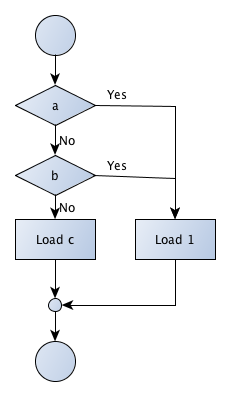
\includegraphics[scale=.5]{images/OrChain.png}
\end{center}
\caption{Program flow of an or chain}
\label{fig:orchain}
\end{figure}

\lstset{language=[x86masm]Assembler, morekeywords={LV,TJMP,LIT}}

\begin{lstlisting}[float,caption={Assembler code of or-chain}, captionpos=b,label=cod:orchain]
...
LV 0, 32		; load value a
TJMP 8			; if true, jump to the end
LV 0, 36		; load value b
TJMP 8			; if true, jump to the end
LV 0, 40		; load value c
JMP 9				; result is determined by c only
LIT 1
...
\end{lstlisting}
When generating this kind of code, we have to deal with the situation that the final addresses we have to jump to are not known in prior. Therefore, we have to construct a so-called or-chain, which work as follows. While parsing a conditional expression, we maintain an int variable holding the 

The translation of {\em and-}expressions works analogously.

\section{Jumps in If- and While-Statements}

\chapter{Error Handling}
ErrorHandler.getInstance().raise(new ...));

\chapter{Attributed Grammar}
\begin{atg}[4.5cm]
\leongage &=& & \semantics{\begin{sem} \newline EmitOp(INC); \newline Emit2(0); \newline int inc\_addr = 1; \newline \end{sem}}\\
&&Stat ";" \{Stat ";"\}. \\

Stat & = & ident ":=" \atgsy{Expr}{\outattr op}  \alternative \\
&& "PUT" \atgsy{Expr}{\outattr op}. \\

\atgsy{Term}{\outattr op} &=& \atgsy{Fact}{\outattr op}  \\
&& \{("*" &\semantics{\begin{sem} opcode = mul \end{sem}}\\
&& \alternative "/" & \semantics{\begin{sem} opcode = div \end{sem}}\\
&&) & \semantics{\begin{sem}EmitOp(\inattr opcode)\end{sem}}\\
&&\atgsy{Fact}{\outattr op} & \semantics{\begin{sem}LoadVal(\inattr op)\end{sem}}
\end{atg}

\bibliography{my_bibliography}{}
\bibliographystyle{alphaurl} % save alternatives are abbrvurl	alphaurl	plainurl	unsrturl

\end{document}  